\documentclass{article}

\usepackage{graphicx}
\usepackage{caption}
\usepackage{subcaption}

\begin{document}

\begin{figure}

        \centering
        
        \begin{subfigure}[b]{0.3\textwidth}
                \centering
                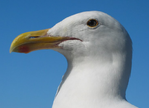
\includegraphics[width=\textwidth]{Figs/subfig1}
                \caption{A gull}
                \label{fig:gull}
        \end{subfigure}%
        ~ %add desired spacing between images, e. g. ~, \quad, \qquad etc.
          %(or a blank line to force the subfigure onto a new line)
        \begin{subfigure}[b]{0.3\textwidth}
                \centering
                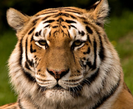
\includegraphics[width=\textwidth,trim=0 10px 0 0,clip=true]{Figs/subfig2}
                \caption{A tiger}
                \label{fig:tiger}
        \end{subfigure}
        
        \begin{subfigure}[b]{0.3\textwidth}
                \centering
                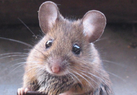
\includegraphics[width=\textwidth]{Figs/subfig3}
                \caption{A mouse}
                \label{fig:mouse}
        \end{subfigure}
        
        \caption{Pictures of animals}
        \label{fig:animals}
        
\end{figure}

\end{document}
